\documentclass[fontsize=11pt,
  paper=a4paper,
  twoside,
  captions=tableheading,
  index=totoc,
  hyperref]{labbook}

\usepackage[bottom=10em]{geometry}
\usepackage[spanish]{babel}
\usepackage[utf8]{inputenc}
\usepackage[T1]{fontenc}
\usepackage[osf]{mathpazo}
\linespread{1.05}\selectfont
\usepackage[scaled=.88]{beramono}
\usepackage[scaled=.86]{berasans}
\usepackage{booktabs,array}
\usepackage{biblatex}
\usepackage{amsmath}
\usepackage{graphicx}
\usepackage{etoolbox}
\usepackage[norule]{footmisc}
\usepackage{lastpage}
\usepackage[dvipsnames]{xcolor}
\definecolor{titleblue}{rgb}{0.16,0.24,0.64}
\definecolor{linkcolor}{rgb}{0,0,0.42}
\addtokomafont{title}{\Huge\color{titleblue}}
\addtokomafont{chapter}{\color{OliveGreen}}
\addtokomafont{section}{\color{Sepia}}
\addtokomafont{pagehead}{\normalfont\sffamily\color{gray}}
\addtokomafont{caption}{\footnotesize\itshape}
\addtokomafont{captionlabel}{\upshape\bfseries}
\addtokomafont{descriptionlabel}{\rmfamily}
\setcapwidth[r]{10cm}
\setkomafont{footnote}{\sffamily}
\deffootnote[4cm]{4cm}{1em}{\textsuperscript{\thefootnotemark}}
\DeclareFixedFont{\textaut}{T1}{phv}{bx}{n}{0.8cm}
\usepackage[nouppercase,headsepline]{scrlayer-scrpage}
\pagestyle{scrheadings}
\clearscrheadfoot

\automark[chapter]{chapter}
\ohead{\headmark}

\setlength{\headheight}{25pt}
\setheadsepline{.4pt}
\addtokomafont{headsepline}{\color{lightgray}}

\ofoot[\normalfont\normalcolor{\thepage\ |\  \pageref{LastPage}}]{\normalfont\normalcolor{\thepage\ |\  \pageref{LastPage}}}
\makeatletter
\patchcmd{\addchap}{\if@openright\cleardoublepage\else\clearpage\fi}{\par}{}{}
\makeatother
\renewcommand*{\chapterpagestyle}{scrheadings}

\usepackage{chngcntr}
\counterwithout{figure}{labday}
\counterwithout{equation}{labday}

\usepackage[
  pdfauthor={Rodriguez S, Torres L, Avila J},
  pdftitle={Laboratory Journal},
  pdfsubject={Couple Oscillators},
  bookmarksopen=true,
  linktocpage=true,
  urlcolor=linkcolor,
  citecolor=linkcolor,
  linkcolor=linkcolor,
  pdfpagelabels=true,
  plainpages=false,
  colorlinks=true,
  bookmarks=true,
  pdfview=FitB]{hyperref}

\usepackage[stretch=10]{microtype}

%----------------------------------------------------------------------------------------
%	DEFINITION OF EXPERIMENTS
%----------------------------------------------------------------------------------------

% Template: \newexperiment{<abbrev>}[<short form>]{<long form>}
% <abbrev> is the reference to use later in the .tex file in \experiment{}, the <short form> is only used in the table of contents and running title - it is optional, <long form> is what is printed in the lab book itself

\newexperiment{example}[Example experiment]{This is an example experiment}
\newexperiment{example2}[Example experiment 2]{This is another example experiment}
\newexperiment{example3}[Example experiment 3]{This is yet another example experiment}

\newsubexperiment{subexp_example}[Example sub-experiment]{This is an example sub-experiment}
\newsubexperiment{subexp_example2}[Example sub-experiment 2]{This is another example sub-experiment}
\newsubexperiment{subexp_example3}[Example sub-experiment 3]{This is yet another example sub-experiment}

%----------------------------------------------------------------------------------------

\begin{document}

%----------------------------------------------------------------------------------------
%	TITLE PAGE
%----------------------------------------------------------------------------------------

\title{\fontsize{40pt}{40pt}\selectfont{Osciladores Acoplados \\[1cm]
\textaut{Bitácora de laboratorio}}}

\author{
  \textaut{Sebastian Rodriguez} \and \textaut{Laura Torres}
  \and \textaut{Julian Avila}
}
\date{}

\maketitle

\printindex
\tableofcontents
\newpage

\begin{addmargin}[4cm]{0cm}

\pagestyle{scrheadings}

%----------------------------------------------------------------------------------------
%	LAB BOOK CONTENTS
%----------------------------------------------------------------------------------------

\labday{Miércoles 23, Abril 2025}


\labday{Miércoles 24, Abril 2025}

El día de hoy se realizo el desarrollo teorico del problema de los tres pendulos físicos, acoplados por los resortes, donde el sistema es el siguiente:
\begin{figure}[h!]

 
  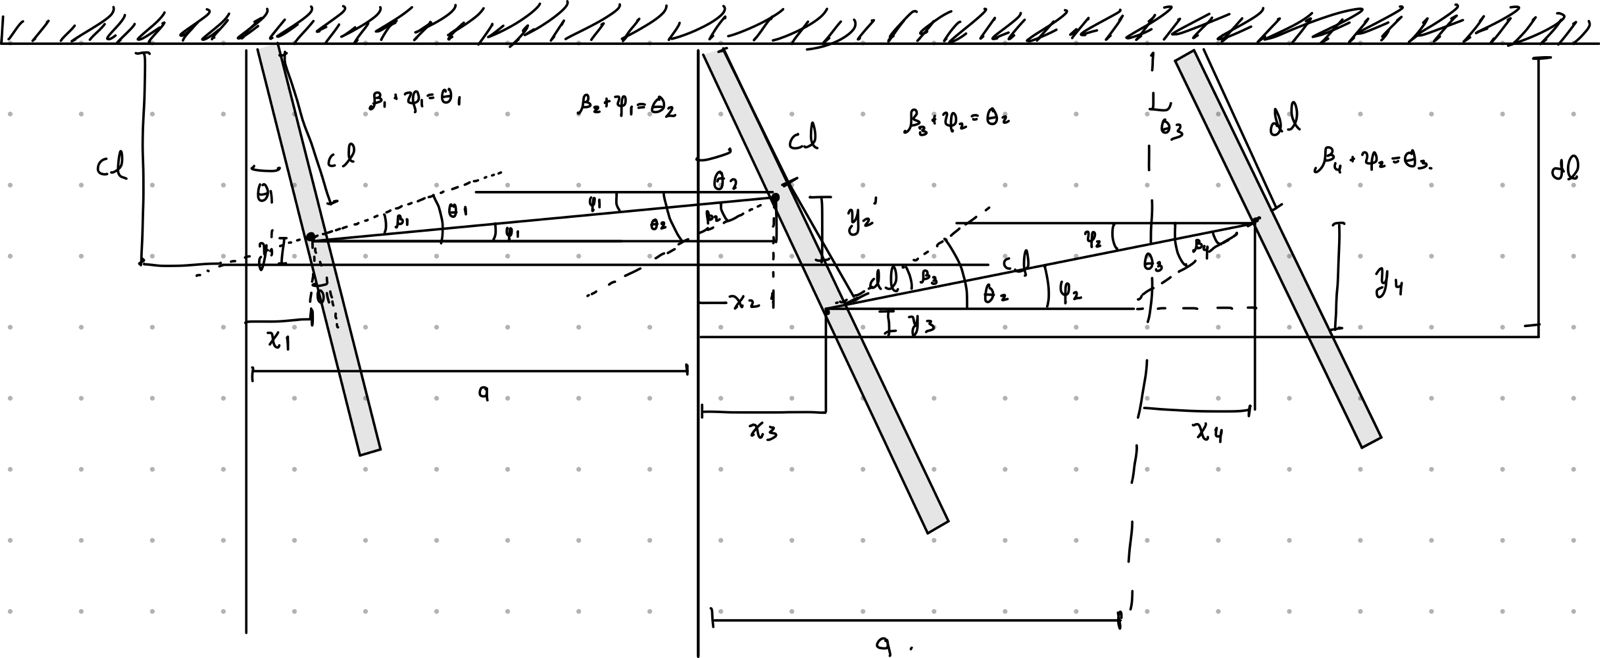
\includegraphics[width=0.8\textwidth]{Figures/IM1.jpeg}

  \caption{Sistema de tres péndulos físicos acoplados por resortes.}
  \label{fig:sistema_pendulos}
\end{figure}
Donde el resultado de la sumatoria de torques para cada pendulo genera el siguiente sistema de ecuaciones:

\begin{equation}
\begin{aligned}
  \ddot{\theta}_1 =\; & \theta_1 \left( \frac{(cl)^2 - x_{cm1} m_1 g}{I_1} \right) + \theta_2 \left( -\frac{k_1 (cl)^2}{I_1} \right) \\
  \ddot{\theta}_2 =\; & \theta_1 \left( \frac{k_1 (cl)^2}{I_2} \right) + \theta_2 \left( -\frac{k_1 (cl)^2}{I_2} + \frac{k_2 (dl)^2}{I_2} + \frac{x_{cm2} m_2 g}{I_2} \right) + \theta_3 \left( \frac{k_2 (dl)^2}{I_2} \right) \\
  \ddot{\theta}_3 =\; & \theta_2 \left( \frac{k_2 (dl)^2}{I_3} \right) + \theta_3 \left( -\frac{k_2 (dl)^2}{I_3} - \frac{x_{cm3} m_3 g}{I_3} \right)
  \end{aligned}
\end{equation}






%----------------------------------------------------------------------------------------

\end{addmargin}

%----------------------------------------------------------------------------------------
%	BIBLIOGRAPHY
%----------------------------------------------------------------------------------------

%----------------------------------------------------------------------------------------

\end{document}
